\documentclass[12pt,a4paper]{article}
\usepackage[latin1]{inputenc}
\usepackage{amsmath}
\usepackage{amsfonts}
\usepackage{amssymb}
\usepackage{listings}
\usepackage{color}
\usepackage{hyperref}
\usepackage{graphicx}
\usepackage{prettyref}
\usepackage{cite}
\newrefformat{lst}{Listing \ref{#1}}
\newrefformat{list}{List \ref{#1} on page \pageref{#1}}
\definecolor{lightGray}{gray}{0.95}
\lstset{
backgroundcolor=\color{lightGray},
breaklines=true,
captionpos=b,
frame=single,
keepspaces=true,
keywordstyle=\color{blue},
language=HTML,
morekeywords={created,modified,tags},
numbers=left
}
\usepackage{float}
\newfloat{lablist}{H}{lol}
\floatname{lablist}{List}

\newcommand{\todo}[1]{{\bf TODO: #1}\\
}

\title{Analysis and documentation of a single page application based on TiddlyWiki}
\author{Christian Jurke 898872, Christian Heigele 901361}
\begin{document}
\maketitle
\tableofcontents
\textbf{Pages Min:13 Max:17 }
\section{Introduction 1}
\section{Decomposition of the TiddlyWiki-Architecture 3}
Traditional web applications are bound to HTTP-Concepts, including stateless requests to transfer data. In these applications a state is often emulated by the use of sessions, which need to be handled on the client and especially on the server side.
These restrictions often lead to a fragmented user experience because the user interface is rebuilt on every data transfer.
TW tries to overcome these restrictions and the resulting disadvantages by building on few but basic concepts which loosen the coupling of HTTP and the actual application eliminating the need of state emulation and resulting in a wiki style single page application with the ability to run in an offline environment.
\subsection{Architecture of the single page application TiddlyWiki 1}
TW builds on some basic concepts. First, TW should not be perceived as a dynamic web page like traditional server-side generated web pages. Instead TW can be perceived as an application which is written entirely in JavaScript and uses HTML5 and CSS3 to render a GUI. This way TW can be executed in any JavaScript environment, like a browser or a node.js instance, while keeping the advantages of a simple application.
One of these advantages is, that TW has no need to emulate an application state, like a traditional web application would need to do.

A second concept concerns the storage of the application data. In contrast to a traditional web application, TW doesn't store the data in an external database but simply uses native data structures already existing in JavaScript to store tiddlers, the basic (atomic) element of the TW application, in the memory. Additional core modules provide a way to persist this storage in simple HTML div elements.

Just by building on these simple and basic concepts,
\begin{itemize}
\item TW is able to store application data in a single HTML page by using div elements as data container.
\item TW is able to store application code (JavaScript) in the same single HTML page.
\item TW can be executed in any JavaScript environment like a browser.
\end{itemize}

These points already enable TW to be used as an offline-enabled single file web application.
Also, by using a server side node.js environment, TW can be used as an online web application, just by providing an additional module to persist tiddlers into plain text files and a module syncing the local data store with the node.js server.

%\todo{tiddlers, modules, plugins}
%\todo{in memory datastore (Wiki) and filter as query language}
To understand the architecture of TW, the first important thing to understand is that anything is a tiddler.
Even the application logic is stored in tiddlers that are marked as "application/javascript".
These tiddlers, which contain application logic, are called modules and a CommonJS compatible module system is responsible for assembling the individual modules into the TW application.
The result is a tree representing the whole TW application containing module tiddlers, data tiddlers and some JavaScript functions and objects.

Only a small part of the TW is not managed as tiddlers, the boot kernel.
The boot kernel is the first thing running, when the application is started and it puts some initial objects and functions into the application tree, which are needed to load and manage tiddlers.
After the boot kernel built this initial application tree, the remaining parts of the application can be loaded as module tiddlers.
Beside some utility functions the most important object that is contributed by the boot kernel is "\$tw.wiki", consisting of JavaScript structures and functions that are used to store and manage the loaded tiddlers.
Among other things this store can be used to add new tiddlers, remove tiddlers and retrieve tiddlers by name.

%\todo{data persistence (saver and deserializer)}
The next important part of the application are deserializers. Deserializers are responsible to load tiddlers from various sources. One of the deserializers provided by the boot kernel for example can load new tiddlers from the current DOM tree.
The counter part of the deserializers are savers and syncadapters.
Both are used to persist the changes made to the store but they work in slightly different ways.
A syncadapter registers at the store for changes.
Now when a tiddler is changed and these changes are written to the store, the syncadapter is triggered and persists the new changes, for each tiddler individually.
If no syncadapter is available a saver can be used to persist new changes.
A saver does not register to change events and so it does not persist each tiddler, when it is changed.
A saver is used to save the complete store or the complete TW for that matter at once. After a user made changes to some tiddlers, this method can be used to download the current state of the store as a completely new TW application.

%\todo{interpreting wiki text (parser)}
%\todo{ui (widgets, dom tree)}
%\todo{sync data store with ui - selective update}
Following the "anything is a tiddler" concept, even the UI consists of tiddlers.
This is possible because tiddlers can not only contain plain text or JavaScript (modules) but the also can contain a special markup text called WikiText.
By using WikiText the user can put markup elements like tables or images in a tiddler.
To provide some more sophisticated UI elements, WikiText can also contain special widgets like text input fields,
checkboxes, dynamic lists etc.
In most cases, these widgets are used to directly modify or represent the information contained in other tiddlers.
If a tiddler is changed and this change should reflect in the UI e.g. a widget, a process called selective update takes place. Selective updating means when a tiddler or a set of tiddlers changes, each widget is asked, if changes to this tiddlers would affect its appearance. If so, the respective widget is re-rendered otherwise it remains unchanged.

The whole application is basically built from three parts. At first, the boot kernel provides the basic functionality to handle tidlers. The second part are tiddlers representing core functionality. These are for example modules which extend the store by more sophisticated functions, UI tiddlers and widget modules, a WikiText parser, sophisticated deserializers, savers, syncadapters, etc.
At this stage the application can be extended by plug-ins. Consequently, a plug-in is a single tiddler which itself contains multiple tiddlers, forming the plug-in. Each of this tiddler might be a module providing new functionality (i.e. a module tiddler marked with "module-type: saver" can extend the application with new methods of saving the current wiki state.).
Also, a tiddler contained in a plug-in can supersede" an existing tiddler and take its place.

By managing nearly every part of the application as tiddlers, the application is only needed to provide some basic functionality to manage the individual tiddlers, load and persist them, render them to HTML output and provide a way to register for the changes made to tiddlers.
This way the whole wiki application can be build from these simple concepts.
Plug-ins can be used to add new functionality to the existing modules or even to replace individual tiddlers/modules,
enabling developers to build whole new applications upon the TW base system.

\begin{figure}[hbtp]
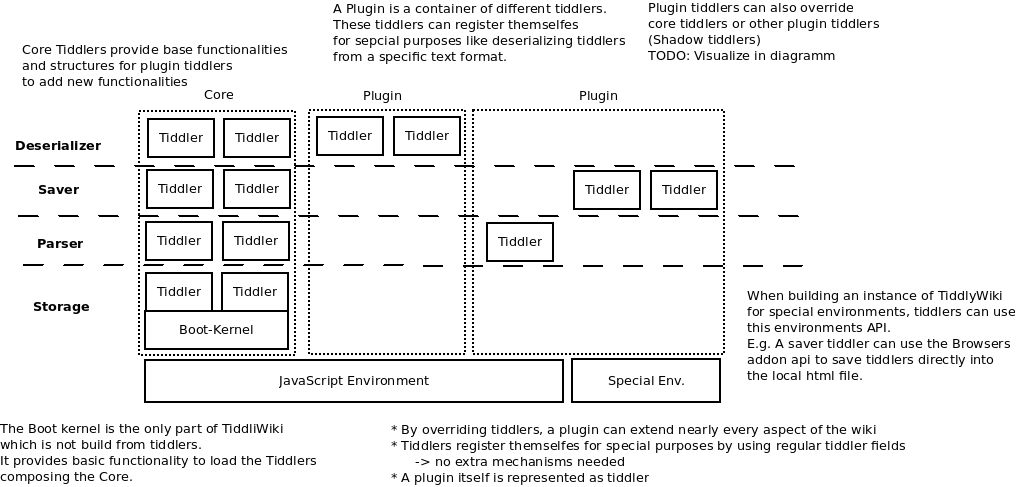
\includegraphics[scale=0.4]{images/overview.png}
\caption{Decomposition of TW}
\end{figure}
\newpage
\subsection{Tiddler as the key element 1}
%\todo{What are the parts of a tiddler - pretty much done}
%\todo{what can a tiddler be - plain text, module, image, container for tiddlers(plugin), ui-element}
\todo{what can i do with tiddlers? - tags, filter-language, widgets modify or represent tiddlers/listoftiddlers}
\todo{example of the concepts power: drag and drop functionality - By providing the functionality to drag and drop a tiddler from one browser to another, we can transfer anything from one tw-instance to another, including plain text, images, new modules like widgets or savers, and even a whole plug-in can be added to an existing TW instance just by draggin and dropping}

A tiddler is the smallest unit of the TiddlyWiki system. It can contain any data like plain text, WikiText markup, JavaScript code (module tiddler), JSON structures\footnote{JSON structures might even contain additional tiddlers. Plug-ins are implemented this way to pack multiple tiddlers in a single plug-in tiddler.}, images in SVG format or even binary images encoded with base64.
Internally Tiddlers are immutable (are they?) objects containing a bunch of key:value pairs called fields. The only required field of a tiddler is the title field. The Standard fields of a tiddler are listed below. Nearly everything in TiddlyWiki is loaded as tiddlers. Plugins for example are a bunch of tiddlers that are distributed as a single JSON tiddler. The only exception is the boot kernel which isn't a tiddler.
\begin{lablist}
\caption{Custom fields of a tiddler div}
\label{list:TiddlerFields}
\begin{description}
\item[created] Timestamp number of milliseconds since 01.01.1970.
\item[modified] Timestamp number of milliseconds since 01.01.1970.
\item[tags] list of tags seperated by whitespace. Tags which contain whitespaces are wrapped by [[ ]], e.g. [[example Tag]].
\item[type] Type of the Tiddler, e.g. text/plain or text/vnd.tiddlywiki .
\item[title] Title of the Tiddler
\item[list] An ordered list of tiddler titles associated with a tiddler
\end{description}
\end{lablist}
\newpage
\subsection{The WikiText concept 1}
The WikiText is a markup language, created especially for the requirements of the TiddlyWiki application. It is based on Markdown\footnote{\url{http://daringfireball.net/projects/markdown/}}, but extended with some TiddlyWiki specific features.  On one hand its a text-to-HTML conversion language and on the other hand its used to provide the interactive features of TiddlyWiki. The aim of this language is to allow the user of the software to focus on the writing.\cite{TIDD:WIKITEXT} The WikiText is used to format Tiddlers within the TiddlyWiki application. The tags of the WikiText syntax can be used within the standard text input field. 
During the saving process these tags renders to HTML elements for example:
\begin{lstlisting}[caption={Example use of WikiText},label=lst:data-div]
WikiText:--- 
Renders as:
HTML:<hr>
WikiText:[img[http://tiddlywiki.com/favicon.ico]]
Renders as: 
HTML:<img src="http://tiddlywiki.com/favicon.ico">
\end{lstlisting}
Furthermore the WikiText is used to access the widgets which are integrated in the application.These widgets are used to enhance the the WikiText with a rich functionality. Widgets are based on the HTML-Syntax but always starts with a \$.
\begin{lstlisting}[caption={Example use of widgets within WikiText},label=lst:data-div]
WikiText:
<$button message="tw-close-tiddler">Close Me!</$button> 
\end{lstlisting}
\section{Bootstrap-Process 2-3}
\subsection{The Heart of TiddlyWiki (Boot-Kernel) 1 - 1.5}
\subsection{Timeline of the startup Process 1 - 1.5}

\section{The Plugin and Module concept 4-5}
\subsection{Introduction to the Plugin-Concept 1}
\subsection{Kernel-Plugins 1}
\subsection{UI-Elements 1}
\subsection{Developing a own Plugin 1-2}
\newpage
\section{The TiddlyWiki data management concept 2-3}
This section descripes how the data of the wiki is stored within Tiddlywiki during the runtime. And how the complete wiki is persistet.
\subsection{Data Management during Runtime 1-2}
During the runtime the data of Tiddlywiki is stored in javascript objects. These objects are synchronized with the DOM-Representation of Tiddlywiki. This means every change of the original data of a Tiddler, fires an event which changes all DOM-Representations of the Tiddler and the javascript object. The barbone Wiki store is created during the boot process and is kept in a object called \$tw.Wiki. This object contains amongst others a hashmap of the different Tiddlers of Tiddlywiki. The Hashmap is used to store the javascript object representation of the different Tiddlers.
\newpage 
\subsection{Data Persistence 1}
\subsubsection*{Persist data}
TiddlyWiki supports a wide range of methods to persist your data. One of this methods is the HTML5 fallback saver. This methods works on almost every browser. With this method a copy of the entire wiki will be downloaded by the browser. This means you get a new file everytime you hit the save button. To avoid this there a some plugins for different browsers to allow to save direct to the current open TiddlyWiki-File.
\subsubsection*{Data-Storage}
TiddlyWiki persists the data within the HTML-File in two Div-Areas depending on whether the encryption of the TiddlyWiki is activated or not. If the TiddlyWiki is not encrypted the data is stored in the Div-Area called ``StoreArea''. Every created Tiddler is stored in a own Div-area with a few custom values. An example of a saved Tiddler is shown below (\prettyref{lst:data-div}). 
\begin{lstlisting}[caption={Data-Div},label=lst:data-div]
<div created="20140611153703343" modified="20140611153734589" tags="testTag" testfield="testvalue" title="TestTiddler" type="text/plain">
	<pre>testText</pre>
</div>
\end{lstlisting}
The Div-Area has the same attributes like the standard tillder fields, listed in  (\prettyref{list:TiddlerFields}), all attributes which are not in this list are parsed as a custom field. The only required attribute is the name attribute, all other attributes are optional.\\
With a activated encryption the data is stored in a special Div-Area called ``encryptedStoreArea''. TiddlyWiki uses the Standford JavaScript Crypto Libary\footnote{\url{http://bitwiseshiftleft.github.io/sjcl/}}. The encrypted Tiddlers are saved in a JSON string within this Div-Area.
\newpage
\section{Summary and Conclusion 1-2}
\bibliography{tiddly}
\bibliographystyle{alpha}
\end{document}
